\subsection{Normal Log-PDF}\label{ssec:normal_log_pdf}

\begin{figure*}[t]
    \centering
    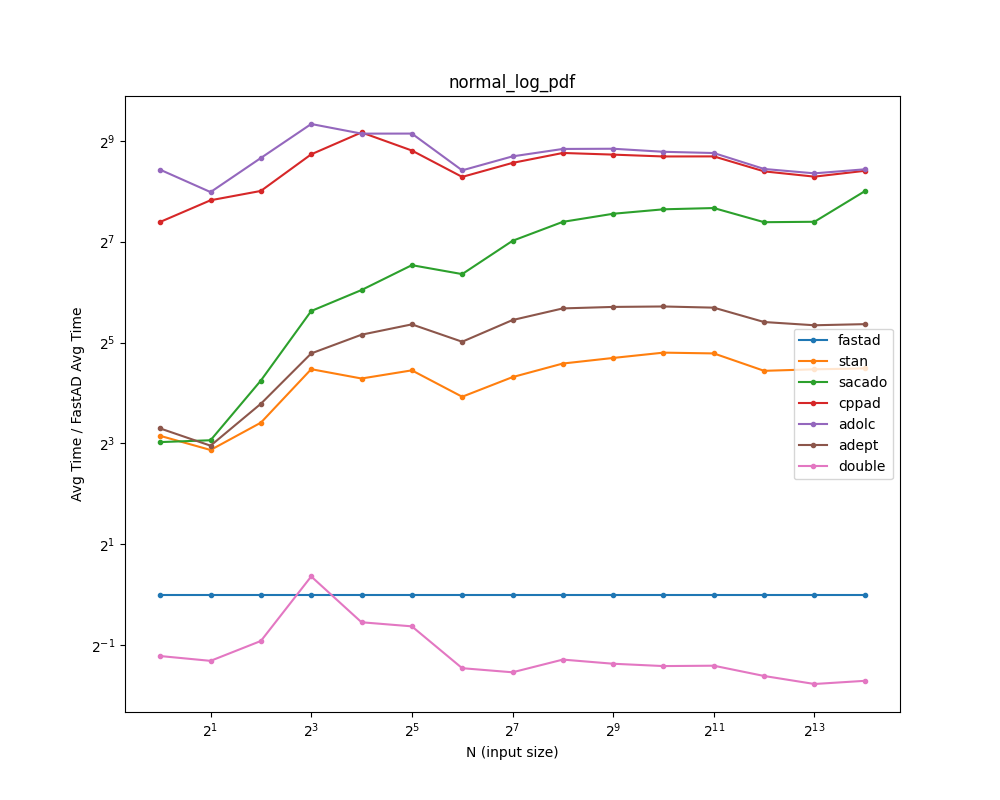
\includegraphics[width=0.7\textwidth]{figs/normal_log_pdf_fig.png}
    \caption{%
        Normal log-pdf benchmark of other libraries against FastAD 
        plotted relative to FastAD average time.
    }\label{fig:normal_log_pdf}
\end{figure*}

The normal log-pdf function is defined up to a constant as:
\[
    f(x) = -\frac{1}{2\sigma^2} \sum\limits_{i=1}^N \paren{x_i - \mu}^2 
           -N\log(\sigma)
\]
For this benchmark, $\mu = -0.56,\,\sigma = 1.37$ and are kept as constants.
Fig.~\ref{fig:normal_log_pdf} shows the benchmark results.

FastAD is the fastest library for all values of $N$.
The trend stabilizes at around $N=2^{7}=128$.
Towards the end, Adept is about $ 9$ times slower,
and Stan about $ 19$ times slower.
Comparing all libraries,
the overall difference we see in this example is the largest we have seen so far,
and this is partly due to how we compute $\log(\sigma)$.
Section~\ref{ssec:compile-time-opt} showed that we can check at compile-time
whether a certain variable is a constant, in which case,
we can perform a more optimized routine.
In this case, since $\sigma$ is a constant, it computes the normalizing constant
$\log(\sigma)$ once and gets reused over multiple AD evaluations 
with no additional cost during runtime,
which saves a lot of time since logarithm is a relatively expensive function.
